%--------------------
% Packages
% -------------------
\documentclass[12pt,a4paper]{article}
% \usepackage[a4paper, left=15mm, right=15mm, top=15mm, bottom=15mm]{geometry}
\usepackage[utf8x]{inputenc}
\usepackage[T1]{fontenc}
%\usepackage{gentium}
\usepackage{mathptmx} % Use Times Font
% \usepackage[siunitx]{circuitikz} % for circuit schematics
\usepackage{siunitx}
\usepackage{amsmath} % for the equation* environment
\usepackage{graphicx}
\usepackage{pgfplots}
\pgfplotsset{compat=1.14}
\usepackage{float}

\usepackage[pdftex]{graphicx} % Required for including pictures % clashes with circuitikz
% \usepackage[swedish]{babel} % Swedish translations
\usepackage[pdftex,linkcolor=black,pdfborder={0 0 0}]{hyperref} % Format links for pdf
\usepackage{calc} % To reset the counter in the document after title page
\usepackage{enumitem} % Includes lists

\frenchspacing % No double spacing between sentences
\linespread{1.2} % Set linespace
\usepackage[a4paper, lmargin=0.08\paperwidth, rmargin=0.08\paperwidth, tmargin=0.08\paperheight, bmargin=0.08\paperheight]{geometry} %margins
%\usepackage{parskip}
% \usepackage[all]{nowidow} % Tries to remove widows
\usepackage[protrusion=true,expansion=true]{microtype} % Improves typography, load after fontpackage is selected

\usepackage[inkscapelatex=false]{svg}
\graphicspath{ {./media/} }

% \pagecolor{black}
% \color{white}

\usepackage{setspace}


%-----------------------
% Set pdf information and add title, fill in the fields
%-----------------------
\hypersetup{ 	
pdfsubject = {},
pdftitle = {ee5311-2025-ee24s053-pwc-report-tut3},
pdfauthor = {Karthik B K <ee24s053@smail.iitm.ac.in>}
}

%-----------------------
% Begin document
%-----------------------
\begin{document}

\title{EE5311 \\ Report of Practical Work Conducted for Tutorial 03}
\author{Karthik B K ee24s053}
\maketitle

\section{Experiment 01}
\subsection{Calculations}
\noindent \underline{Sizing the pMOS for Minimum Delay} \newline
In order to minimize propagation delay, we know from the exercises conducted in class that:
\begin{equation}
    W_p = \sqrt{\frac{k_n}{k_p}} \cdot W_n
\end{equation}

\noindent Using this, we obtain $W_p = 0.70 \mu m$. We only want to use multiples of the unit-sized inverter, so we use $W_p = 0.84 \mu m$ instead.\newline \newline 
\noindent \underline{Delay as a function of $V_{DD}$} \newline
\noindent We can compute the delays for the supply voltage in the interval [1V, 1.8V] with the step size of 0.1 V as follows.
\begin{equation}
    t_{p, LH} = \frac{C_{total}(\frac{V_{DD}}{2})(E_{C,p}L+V_{DD}-|V_{T,p}|)}{k_p(\frac{W_p}{L_p})E_{C,p}L(V_{DD} - |V_{T,p}|)^2}
\end{equation}
\begin{equation}
    t_{p, HL} = \frac{C_{total}(\frac{V_{DD}}{2})(E_{C,n}L+V_{DD}-|V_{T,n}|)}{k_n(\frac{W_n}{L_n})E_{C,n}L(V_{DD} - |V_{T,n}|)^2}
\end{equation}
\begin{equation}
    t_p = \frac{(t_{p,LH} + t_{p,HL})}{2}
\end{equation}
\noindent We obtain the following delay values.
\begin{filecontents}{dly.dat}
X   $V_{DD}$    $t_{p,LH}$  $t_{p,HL}$  $t_{p}$     $EDP$
1	1	        1.12E-10	2.38E-11	6.81E-11	1.09E-25
2	1.1	        7.40E-11	2.10E-11	4.75E-11	9.20E-26
3	1.2	        5.60E-11	1.97E-11	3.79E-11	8.72E-26
4	1.3	        4.50E-11	1.90E-11	3.20E-11	8.65E-26
5	1.4         3.78E-11	1.86E-11	2.82E-11	8.85E-26
6	1.5         3.28E-11	1.85E-11	2.56E-11	9.23E-26
7	1.6         2.92E-11	1.85E-11	2.39E-11	9.77E-26
8	1.7         2.65E-11	1.86E-11	2.25E-11	1.04E-25
9	1.8         2.43E-11	1.88E-11	2.16E-11	1.12E-25
\end{filecontents}

\begin{figure}[H]
\centering
\begin{tikzpicture}
\begin{axis}[
axis lines=middle,
ymin=0,
x label style={at={(current axis.right of origin)},anchor=north, below=10mm},
title={\textit{Delay vs $V_{DD}$}},
    xlabel=$V_{DD}$ (V),
  ylabel=Delay (s),
  % xticklabel style = {rotate=30,anchor=east},
  % xticklabel style = {anchor=below},
   enlargelimits = false,
  xticklabels from table={dly.dat}{$V_{DD}$},xtick=data]
\addplot[orange,thin,mark=square*] table [y=$t_{p,LH}$,x=X]{dly.dat};
\addlegendentry{$t_{p,LH}$}
\addplot[blue,thin,mark=square*] table [y=$t_{p,HL}$,x=X]{dly.dat};
\addlegendentry{$t_{p,HL}$}]
\addplot[red,thick,mark=square*] table [y=$t_{p}$,x=X]{dly.dat};
\addlegendentry{$t_{p}$}]
\end{axis}
\end{tikzpicture}
\caption{A plot of propagation delay as a function of supply voltage.}
\end{figure}

\noindent \underline{Energy Delay Product as a function of $V_{DD}$} \newline
\noindent We can compute the Energy Delay Product, EDP as a function of $V_{DD}$ and $t_p$ as follows.
\begin{equation}
    EDP = \frac{1}{2}C_{total}V_{DD}^2t_p
\end{equation}
\noindent We use $C_{total}$ as 3.2 fF, and obtain the following values.
\begin{figure}[H]
\centering
\begin{tikzpicture}
\begin{axis}[
axis lines=middle,
ymin=0,
x label style={at={(current axis.right of origin)},anchor=north, below=10mm},
title={\textit{EDP and Delay vs $V_{DD}$}},
    xlabel=$V_{DD}$ (V),
    ylabel=EDP (J),
    ymin=0.8e-25,
  % xticklabel style = {rotate=30,anchor=east},
  % xticklabel style = {anchor=below},
   enlargelimits = false,
    xticklabels from table={dly.dat}{$V_{DD}$},xtick=data]
% \addplot[orange,thin,mark=square*] table [y=$t_{p,LH}$,x=X]{dly.dat};
% \addlegendentry{$t_{p,LH}$}
% \addplot[blue,thin,mark=square*] table [y=$t_{p,HL}$,x=X]{dly.dat};
% \addlegendentry{$t_{p,HL}$}]
\addplot[red,thin,mark=square*] table [y=$EDP$,x=X]{dly.dat};
\addplot[
    mark=*,
    mark options={fill=red, scale=2},
    mark indices={4}
] table[x=X, y=$EDP$] {dly.dat};

\addlegendentry{$EDP$}]
\end{axis}
% \begin{axis}[
% axis lines=middle,
% ymin=0,
% x label style={at={(current axis.right of origin)},anchor=north, below=10mm},
% title={\textit{EDP and Delay vs $V_{DD}$}},
%     axis y line*=right,
%     axis x line=none,
%     xlabel=$V_{DD}$ (V),
%     ylabel=Delay (s),
%     % xticklabel style = {rotate=30,anchor=east},
%     % xticklabel style = {anchor=below},
%    enlargelimits = false,
% % xticklabels from table={dly.dat}{$V_{DD}$},xtick=data]
% % \addplot[orange,thin,mark=square*] table [y=$t_{p,LH}$,x=X]{dly.dat};
% % \addlegendentry{$t_{p,LH}$}
% % \addplot[blue,thin,mark=square*] table [y=$t_{p,HL}$,x=X]{dly.dat};
% % \addlegendentry{$t_{p,HL}$}]
% \addplot[blue,thick,mark=square*] table [y=$EDP$,x=X]{dly.dat};
% \addlegendentry{$EDP$}]
% \end{axis}
\end{tikzpicture}
\caption{A plot of EDP as a function of supply voltage.}
\end{figure}

\subsection{Schematics}
\noindent We draw the following schematics for an inverter using \emph{xschem}.
\begin{center}
\begin{tabular}{cc}
     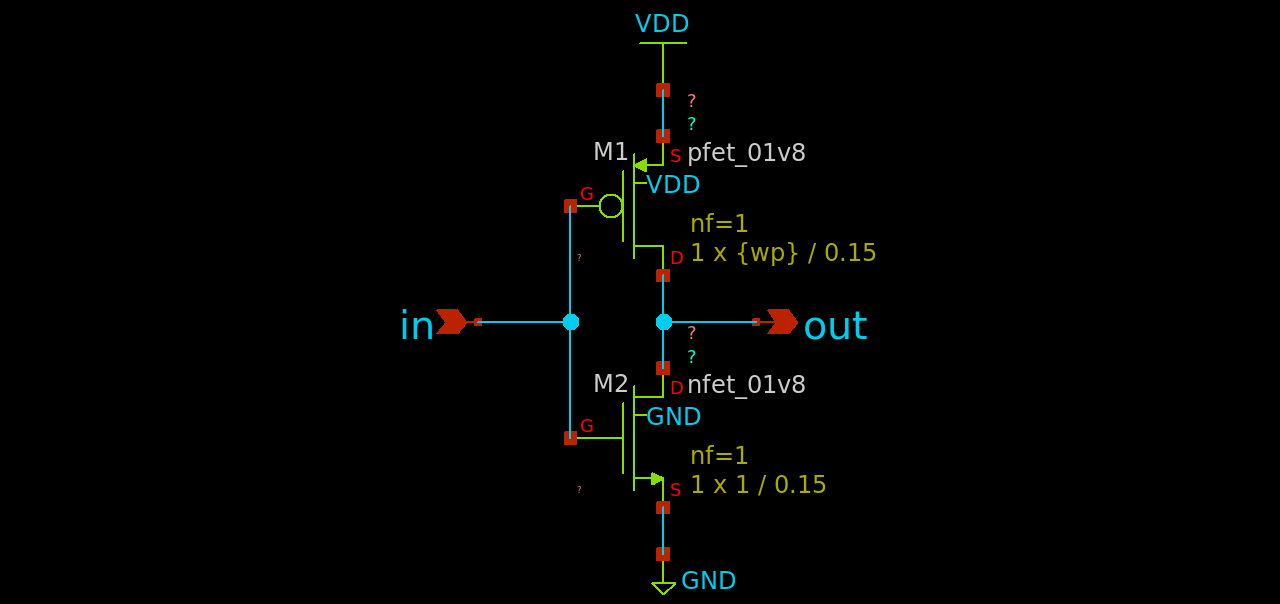
\includegraphics[width=0.40\linewidth]{tut3/reports/media/inv.png} &
     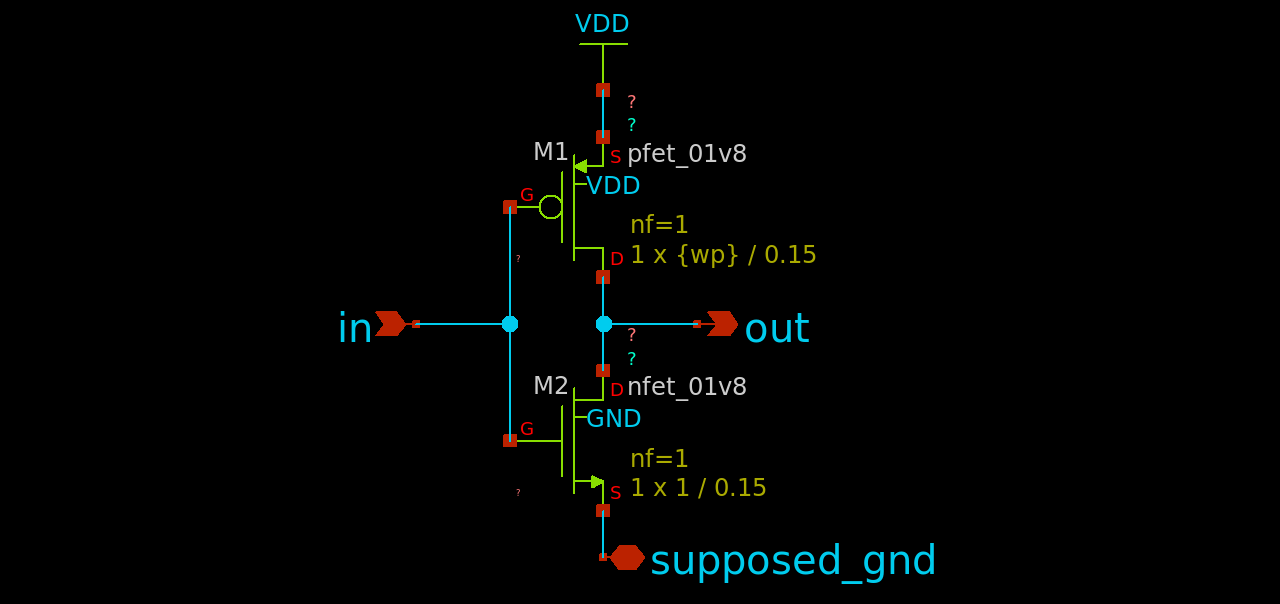
\includegraphics[width=0.40\linewidth]{tut3/reports/media/inv_nognd.png} \\
     Fig 1a: A static CMOS inverter & Fig 1b: An inv with the ground pin exposed
\end{tabular}
\\
\begin{tabular}{cc}
     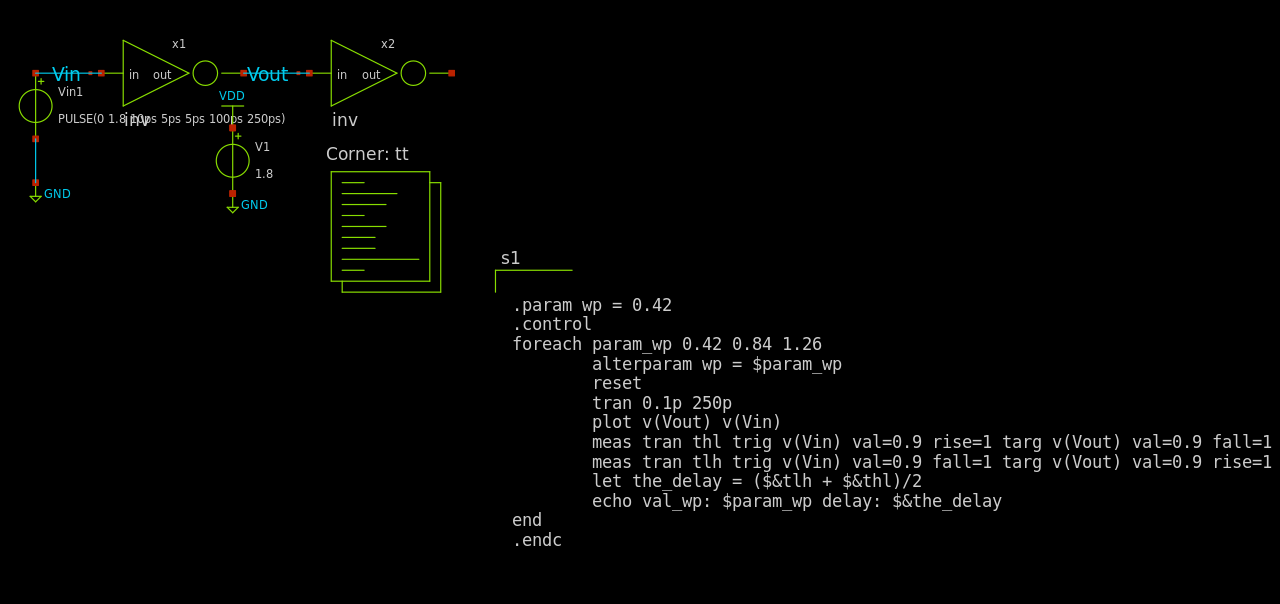
\includegraphics[width=0.40\linewidth]{tut3/reports/media/expt1_a.sch.png} &
     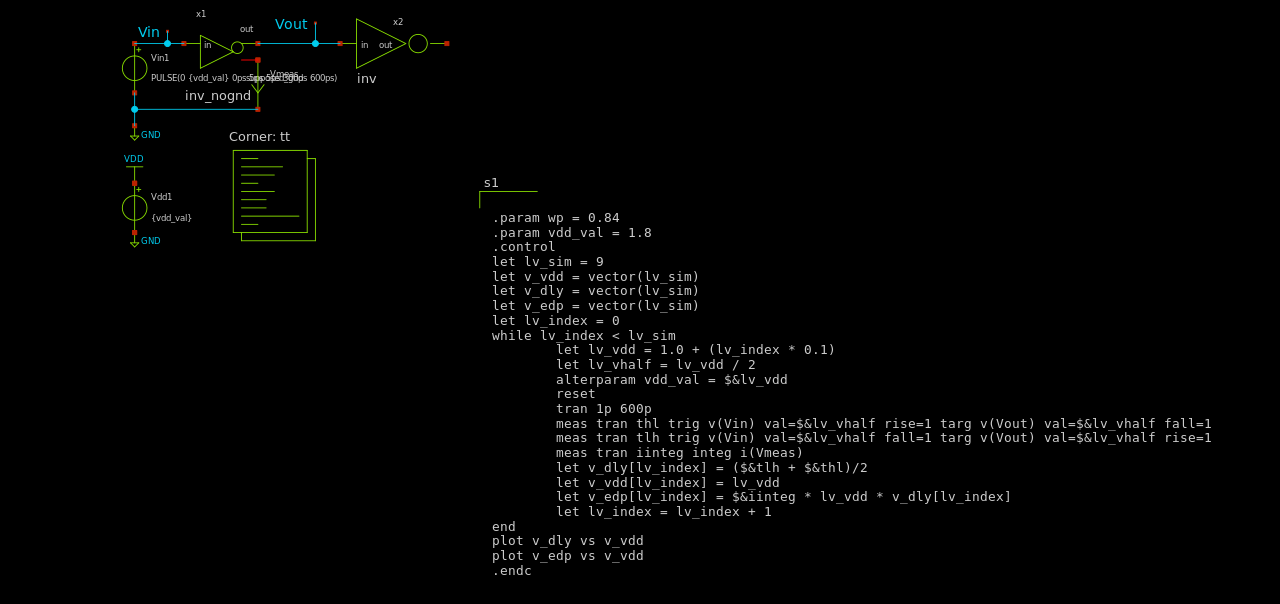
\includegraphics[width=0.40\linewidth]{tut3/reports/media/expt1_b.sch.png} \\
     Fig 1c: Simulation Setup 1 & Fig 1d: Simulation Setup 2
\end{tabular}
\end{center}

\subsection{Measurements}
\noindent We perform a transient simulation for the simulation setup shown in Fig 1c,  for three sizes of pMOS, and obtain the following plots.
\begin{center}
\begin{tabular}{cc}
     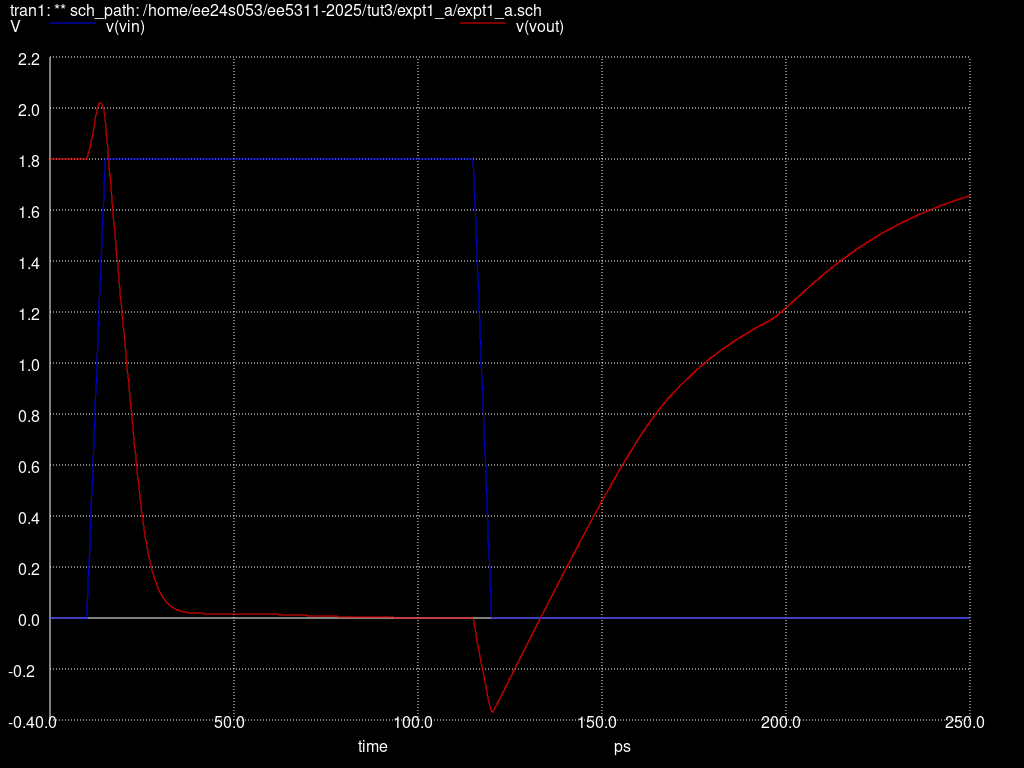
\includegraphics[width=0.40\linewidth]{tut3/reports/media/expt1a_dly_2.png} &
     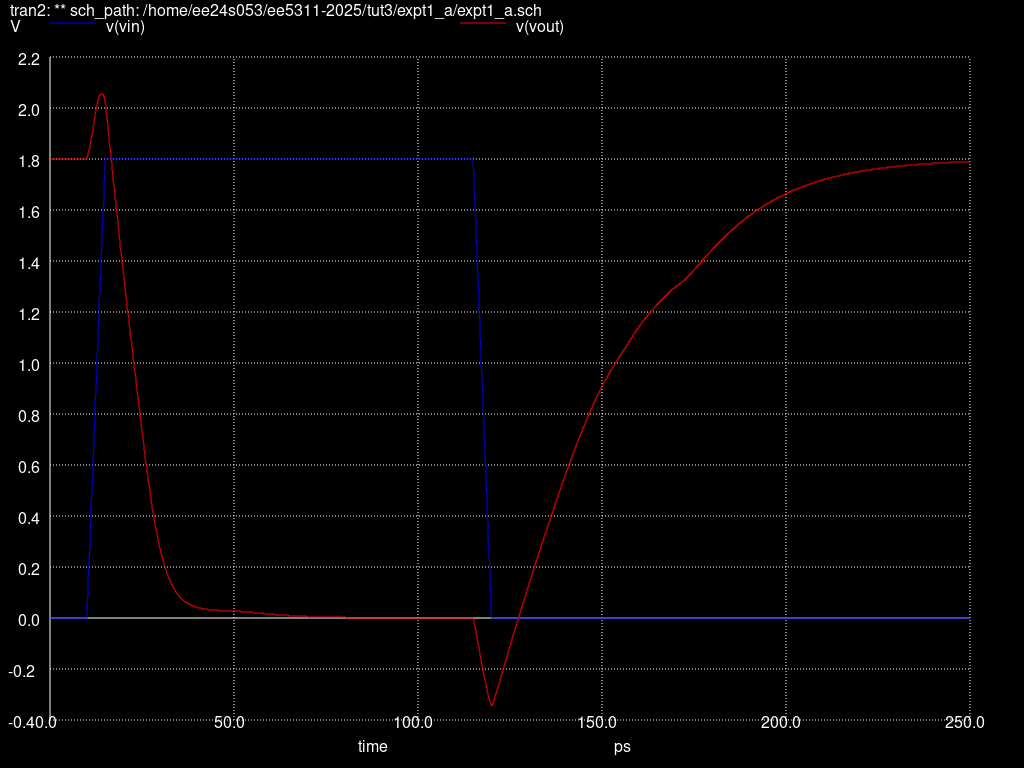
\includegraphics[width=0.40\linewidth]{tut3/reports/media/expt1a_dly_1.png} \\
     Fig 1a: $W_p = 0.42 \mu m$ & Fig 1b: $W_p = 0.84 \mu m$
\end{tabular}
\\
\begin{tabular}{cc}
     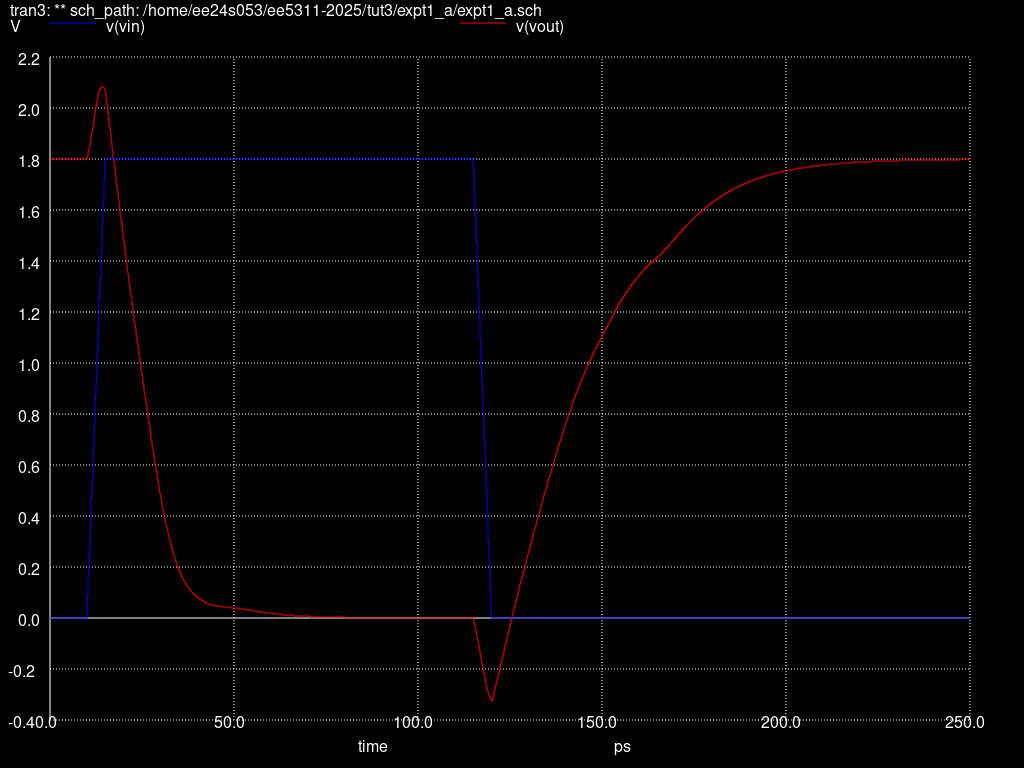
\includegraphics[width=0.40\linewidth]{tut3/reports/media/expt1a_dly_0.png} \\
     Fig 1c: $W_p = 1.26 \mu m$
\end{tabular}
\end{center}
\noindent We then size the pMOS for minumum propagation delay and vary the supply voltage levels from 1V all the way to 1.8V with a step size of 0.1V. We obtain the following plots.
\begin{center}
\begin{tabular}{cc}
     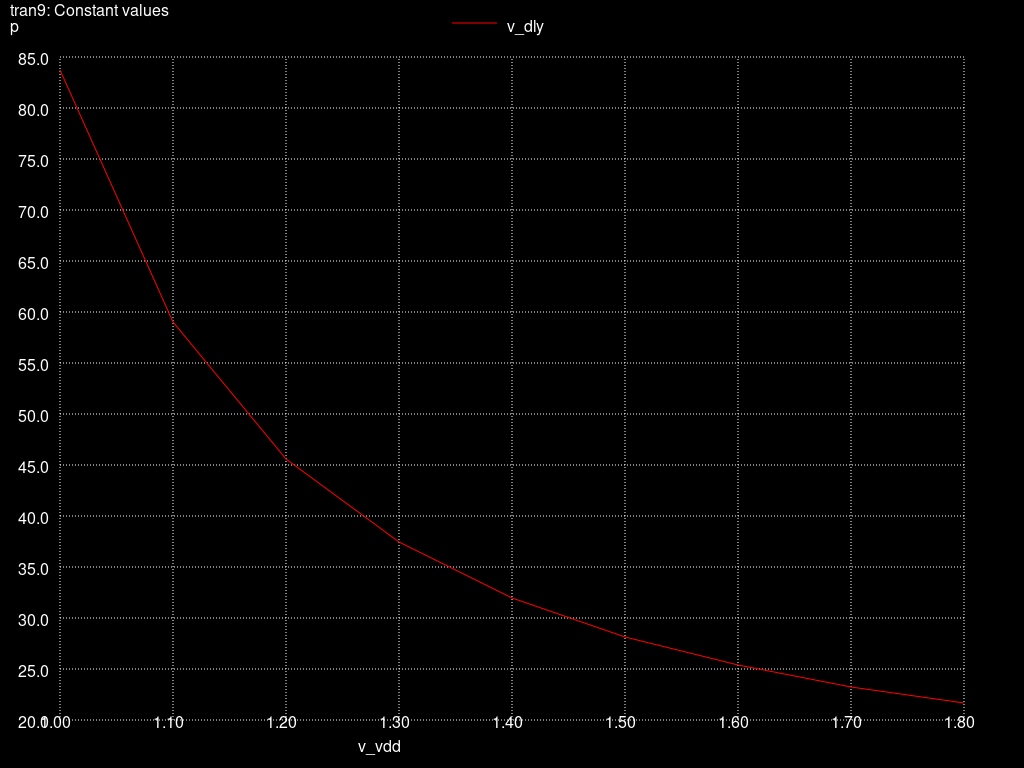
\includegraphics[width=0.49\linewidth]{tut3/reports/media/dly.png} &
     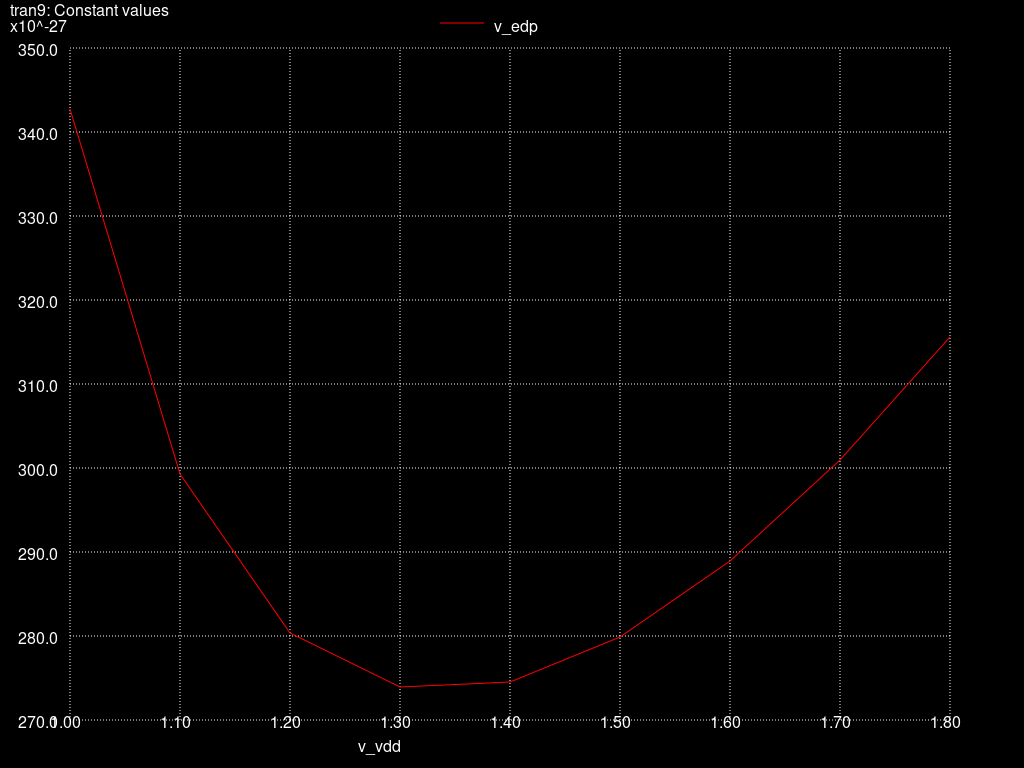
\includegraphics[width=0.49\linewidth]{tut3/reports/media/edp.png} \\
     Fig 1a: Delay & Fig 1b: EDP
\end{tabular}
\end{center}

\noindent From visual inspection, we note that the value of $V_{DD}$ at which the EDP is minimized is 1.3 V. This is expected based on our calculations from earlier. The delay values are also comparable.

\section{Declarations}
\begin{enumerate}
    \item I have hosted this work publicly on github to assist reproducability of all my results. The same can be accessed through the following \href{https://github.com/iamkarthikbk/ee5311-2025}{\underline{link}}.
\end{enumerate}

\end{document}
